\documentclass{foi}
\usepackage[utf8]{inputenc}
\usepackage{lipsum}
\usepackage{float}
\usepackage{hyperref}
\usepackage{enumitem}
\usepackage{longtable}


\DeclareUnicodeCharacter{0140}{l}
\vrstaRada{\diplomski} % \diplomski
\title{Izrada komponente za detekciju označenih odgovora na pismenim ispitima}
\author{Filip Milohanović}
\spolStudenta{\musko} % \zensko ili \musko
\mentor{Marko Mijač}
\spolMentora{\musko} % \zensko ili \musko
\godina{2025}
\mjesec{lipanj}
\date{2025}
%\status{redoviti}
\jmbag{0016148270 }
\smjer{Informacijsko i programsko inženjerstvo} % (ili Poslovni sustavi, Ekonomika poduzetništva, Primjena informacijske tehnologije u poslovanju, Informacijsko i programsko inženjerstvo, Baze podataka i baze znanja, Organizacija poslovnih sustava, Informatika u obrazovanju)
\titulaProfesora{Doc. dr. sc.}

\sazetak{Opsega od 100 do 300 riječi. Sažetak upućuje na temu rada, ukratko se iznosi čime se rad bavi, teorijsko-metodološka polazišta, glavne teze i smjer rada te zaključci.}

\kljucneRijeci{riječ; riječ; ...riječ; Obuhvaća 7+/-2 ključna pojma koji su glavni predmet rasprave u radu.}

\begin{document}

\maketitle

\tableofcontents

\pagestyle{plain}
\chapter{Uvod}

U današnjem obrazovnom sustavu nastavnici provode jako puno vremena na radnim zadacima koji ne podižu kvalitetu obrazovanja već su administrativni i često repetitivni poslovi. Jedan od tih zadataka je ocjenjivanje ispita, pogotovo ako se radi o velikoj količini pristupnika testu. Kod testova s izrazito velikom količinom pristupnika se zato koriste ispiti koji uključuju list za odgovore što olakšava ocjenjivanje. Time se značajno ubrzava cijeli proces ocjenjivanja pošto nije potrebno čitati odgovore koji su u različitim formatima i potencijalno na više stranica, ali i dalje ostaje repetitivni dio posla koji uključuje usporedbu odgovora s rješenjima. Kroz ovaj rad bit će prikazana softverska komponenta otvorenog koda koja rješava ovaj problem tako da naspram slike detektira označene odgovore i ocjenjuje ispit.

Kroz ovaj rad istražuje se razne metode za detektiranje označenih odgovora s ciljem izrade komponente visoke preciznosti, prateći metodologiju znanstvenog oblikovanja.

\chapter{Metode i tehnike rada}

S obzirom na to da se radi o temi koja uključuje obradu slike, što zahtijeva opsežno istraživanje, manipulaciju parametrima i testiranje pristupa odlučeno je koristiti inkrementalan pristup razvoju. Prije same izrade rješenja, provedena je minimalna potrebna količina istraživanja, a zatim se ostatak istraživanja odvijao paralelno s razvojem.

Iterativni razvoj ovog rješenja može se podijeliti u 3 faze: pretprocesiranje, procesiranje i postprocesiranje slike. Jedna od najvažnijih tehnika tijekom razvoja bila je  vizualizacija svakog koraka obrade slike. To je omogućilo izravan uvid u status i smjer razvoja. Time je od samog početka omogućen uvid u mane i prednosti korištenih metoda. Ovo je značajno doprinijelo definiranju budućih razvojnih koraka, poput  dodatnog istraživanja, promjene pristupa i slično. 

Da bi sama vizualizacija bila što učinkovitija korišteno je više različitih fotografija, slikanih u različitim uvjetima. To je omogućilo verifikaciju funkcionalnosti dijelova rješenja na različitim ulaznim podacima od samog početka razvoja, što je značilo da na kraju projekta nije bilo potrebno pokrivati rubne slučajeve jer je rješenje bilo dizajnirano da ih pokriva od samog početka.

Rješenje je izrađeno pomoću .NET tehnologije i C\# programskog jezika u obliku biblioteke, što omogućuje drugim rješenjima jednostavnu integraciju koristeći .dll. 

Kroz ovaj rad nije bio cilj razviti vlastitu biblioteku za računalni vid, već je korištena jedna od postojećih biblioteka otvorenog koda. EmguCv je odabran pošto se radi o .NET omotaču za jednu od najpopularnijih biblioteka za računalni vid OpenCV. Osim toga, rješenje omogućuje korisnicima da koriste alternativnu biblioteku s uvjetom da izrade svoju implementaciju odgovarajućih metoda.

\chapter{Razrada teme}

Kroz teoretski dio rada predočit će se cijeli proces detekcije odgovora na pismenim ispitima koristeći obradu slike pomoću računalnog vida. Analizirat će postojeća rješenja ovog problema koja koriste računalni vid i alternativne pristupe. 

Svi ti pristupi imaju isti cilj, a to je izvlačenje relevantnih podataka iz slike te naknadna obrada tih podataka. U kontekstu ovog rada to bi značilo da se iz slike moraju izvući podaci o označenim odgovorima za određeno pitanje te se ti podaci uspoređuju s listom točnih odgovora. 

\section{Digitalna slika }

Za početak važno je razumjeti što su to digitalne slike i koje sve informacije one sadrže. Digitalna slika je zapravo računalna datoteka koja reprezentira fotografiju pomoću piksela. Piksel je zapravo najmanji element slike koji je reprezentiran s 3 kanala boja: Crvena (R), zelena (G), plava (B) u RGB modelu. Postoje i drugi kanali boja, ali za potrebe ovog rada fokus će biti na RGB modelu. \cite{DigitalnaSlika}.

Sama boja piksela se određuje kombinacijom vrijednosti iz RGB kanala. Dok je sam broj mogućih boja određen brojem bitova koji svaki RGB kanal može poprimiti. Taj koncept se još naziva dubinom boje (\textit{eng. color depth}). Na primjer, pikseli 24-bitne slike mogu poprimiti do 16,777,216 unikatnih boja pošto svaki kanal ima 8 bitova. \cite{DigitalnaSlika}:

\[
\text{Broj boja} = 2^{8} \times 2^{8} \times 2^{8} = 2^{24} = 16.777.216
\]

S pomoću piksela se također može definirati veličinu slike, to jest rezolucija. Rezolucija je sveukupan broj piksela koje neka slika sadrži i izražava se množenjem širine slike s visinom slike:

\[
\text{Ukupan broj pikslea} = \text{Širina} \times \text{Visina}
\]

Za sliku rezolucije $1920 \times 1080$ to je:

\[
\text{Ukupan broj pikslea} = 1920 \times 1080 = 2.073.600 \text{ piksela}
\]

Obično veća rezolucija znači više detalja na slici. Što se više detalja nalazi na slici to su bolje šanse za izvući korisne informacije sa slike. No naravno da rezolucija sama ne određuje kvalitetu digitalne slike, već veliku ulogu igraju i fizički uvjeti u kojima je slika izrađena. Pod to spada osvjetljenje, čistoća kamere, kvaliteta senzora i sl.

Sliku se osim metrika poput dubine boja i rezolucije može opisati i omjerom slike (\textit{eng. aspect ratio}). Omjer slike opisuje odnos broja piksela po širini i visini slike. Omjer slike većinom je vezan za način na koji je slika uslikana ili na način na koji se ona reproducira. Na primjer, profesionalni fotoaparati većinom koriste omjer slike 3:2, kamere pametnih telefona koriste omjer 4:3 dok računalni monitori koriste 16:9 \cite{AspectRatio}.

Važno je napomenuti da se većina do sada spomenutih pojmova odnosi isključivo na slike rasterske grafike, dok za vektorske slike vrijede neki drugi pojmovi i pravila. U ovom radu koristit će se rasterske slike, odnosno slike koje se sastoje od piksela. Za razliku od rasterske grafike, vektorska grafika nije bazirana na pikselima, već je definirana matematičkim funkcijama i krivuljama. To ujedno znači da za nju ne vrijedi pojam rezolucije, budući da njezina kvaliteta nije ograničena statičnim informacijama poput piksela, već se dodatni detalji mogu izračunati iz definiranih funkcija \cite{DigitalnaSlika}.

\subsection{Slike u boji}

Povijest fotografije počinje 1830-ih godina, prve fotografije su bile crno-bijele. No to se već 1861. promijenilo pojavom prve slike u boji. Clerk Maxwell je korištenjem crvenih, zelenih i plavih filtera izradio prvu sliku u boji. Zatim je kompanija Kodak popularizirala slike u boji i danas su one de facto standard. Zatim se s vremenom analogna fotografija razvila u digitalnu fotografiju \cite{ImageHistory}.

Danas većina digitalnih slika koje ljudi stvaraju sadrže boje i koriste sva tri kanala boje. Za razumijevanje ovog rada potrebno je razumjeti kakve informacije sadrži pojedini kanal boje. Svaki kanal predstavlja jednu primarnu boju poput crvene, zelene ili plave. I svaki piksel poprima određenu vrijednost za svaki kanal, ovisno o kombinaciji bitova. Za 24-bitnu sliku svaki kanal ima 8 bitova to jest 256 mogućih vrijednosti. 

To znači da u svakom kanalu postoji vrijednost od 0 do 255 koja definira jačinu svjetlosti za tu primarnu boju. Nulu bi označavala kompletno crna boja dok bi 255 bila potpuno osvijetljena primarna boja,  ovisno o kojem se kanalu radi. Kombinacijom tih 3 kanala se zapravo dobivaju međuboje i time se stvara konačni izgled slike. \cite{GrayscaleSlika}.

\begin{figure}[H]
    \centering
    \includegraphics[width=1.0\linewidth]{slike/Color_chanell_separation.png}
    \caption{Prikaz slike u boji i pripadajućih kanala boja u RGB modelu (vlastita izrada)}
    \label{fig:channels}
\end{figure}

Kao što je prikazano na slici, kanali boja prikazani su kao slike čiji pikseli poprimaju crnu, bijelu i nijanse sive boje. Također kanali se ponekad znaju vizualizirati pomoću primarne boje kanala kojeg reprezentiraju, ali sami podaci koje digitalna slika sadrži su uvijek jednaki, jedino način njihove vizualizacije varira. 

\subsection{Sive slike}

Sive slike (\textit{eng. grayscale}) su poseban tip digitalnih slika koji ima samo jedan kanal boja. U tom kanalu vrijednost piksela reprezentira svjetlinu piksela. Vizualizacija takvih slika poprima boje od bijele do crne uključujući nijanse sive. Na primjer za sliku s dubinom boja od 8 bitova, nula predstavlja crnu boju, 255 prestavlja bijelu boju, a međuvrijednosti su predstavljene nijansama sive boje \cite{GrayscaleSlika}.

Sive slike su jedan od važnijih koncepata obrade slike i računalnog vida. One su zapravo početna točka kod mnogih algoritama za procesiranje slika. Često se koriste kao prvi korak obrade. Izrazito su korisne za detekciju rubova, segmentaciju slike, prepoznavanje uzoraka i slično \cite{Grayscale2}. Kroz rad će se detaljnije prikazati njihova važnost i uloga u kontekstu detektiranja označenih odgovora na pismenim ispitima. 

\begin{figure}[H]
    \centering
    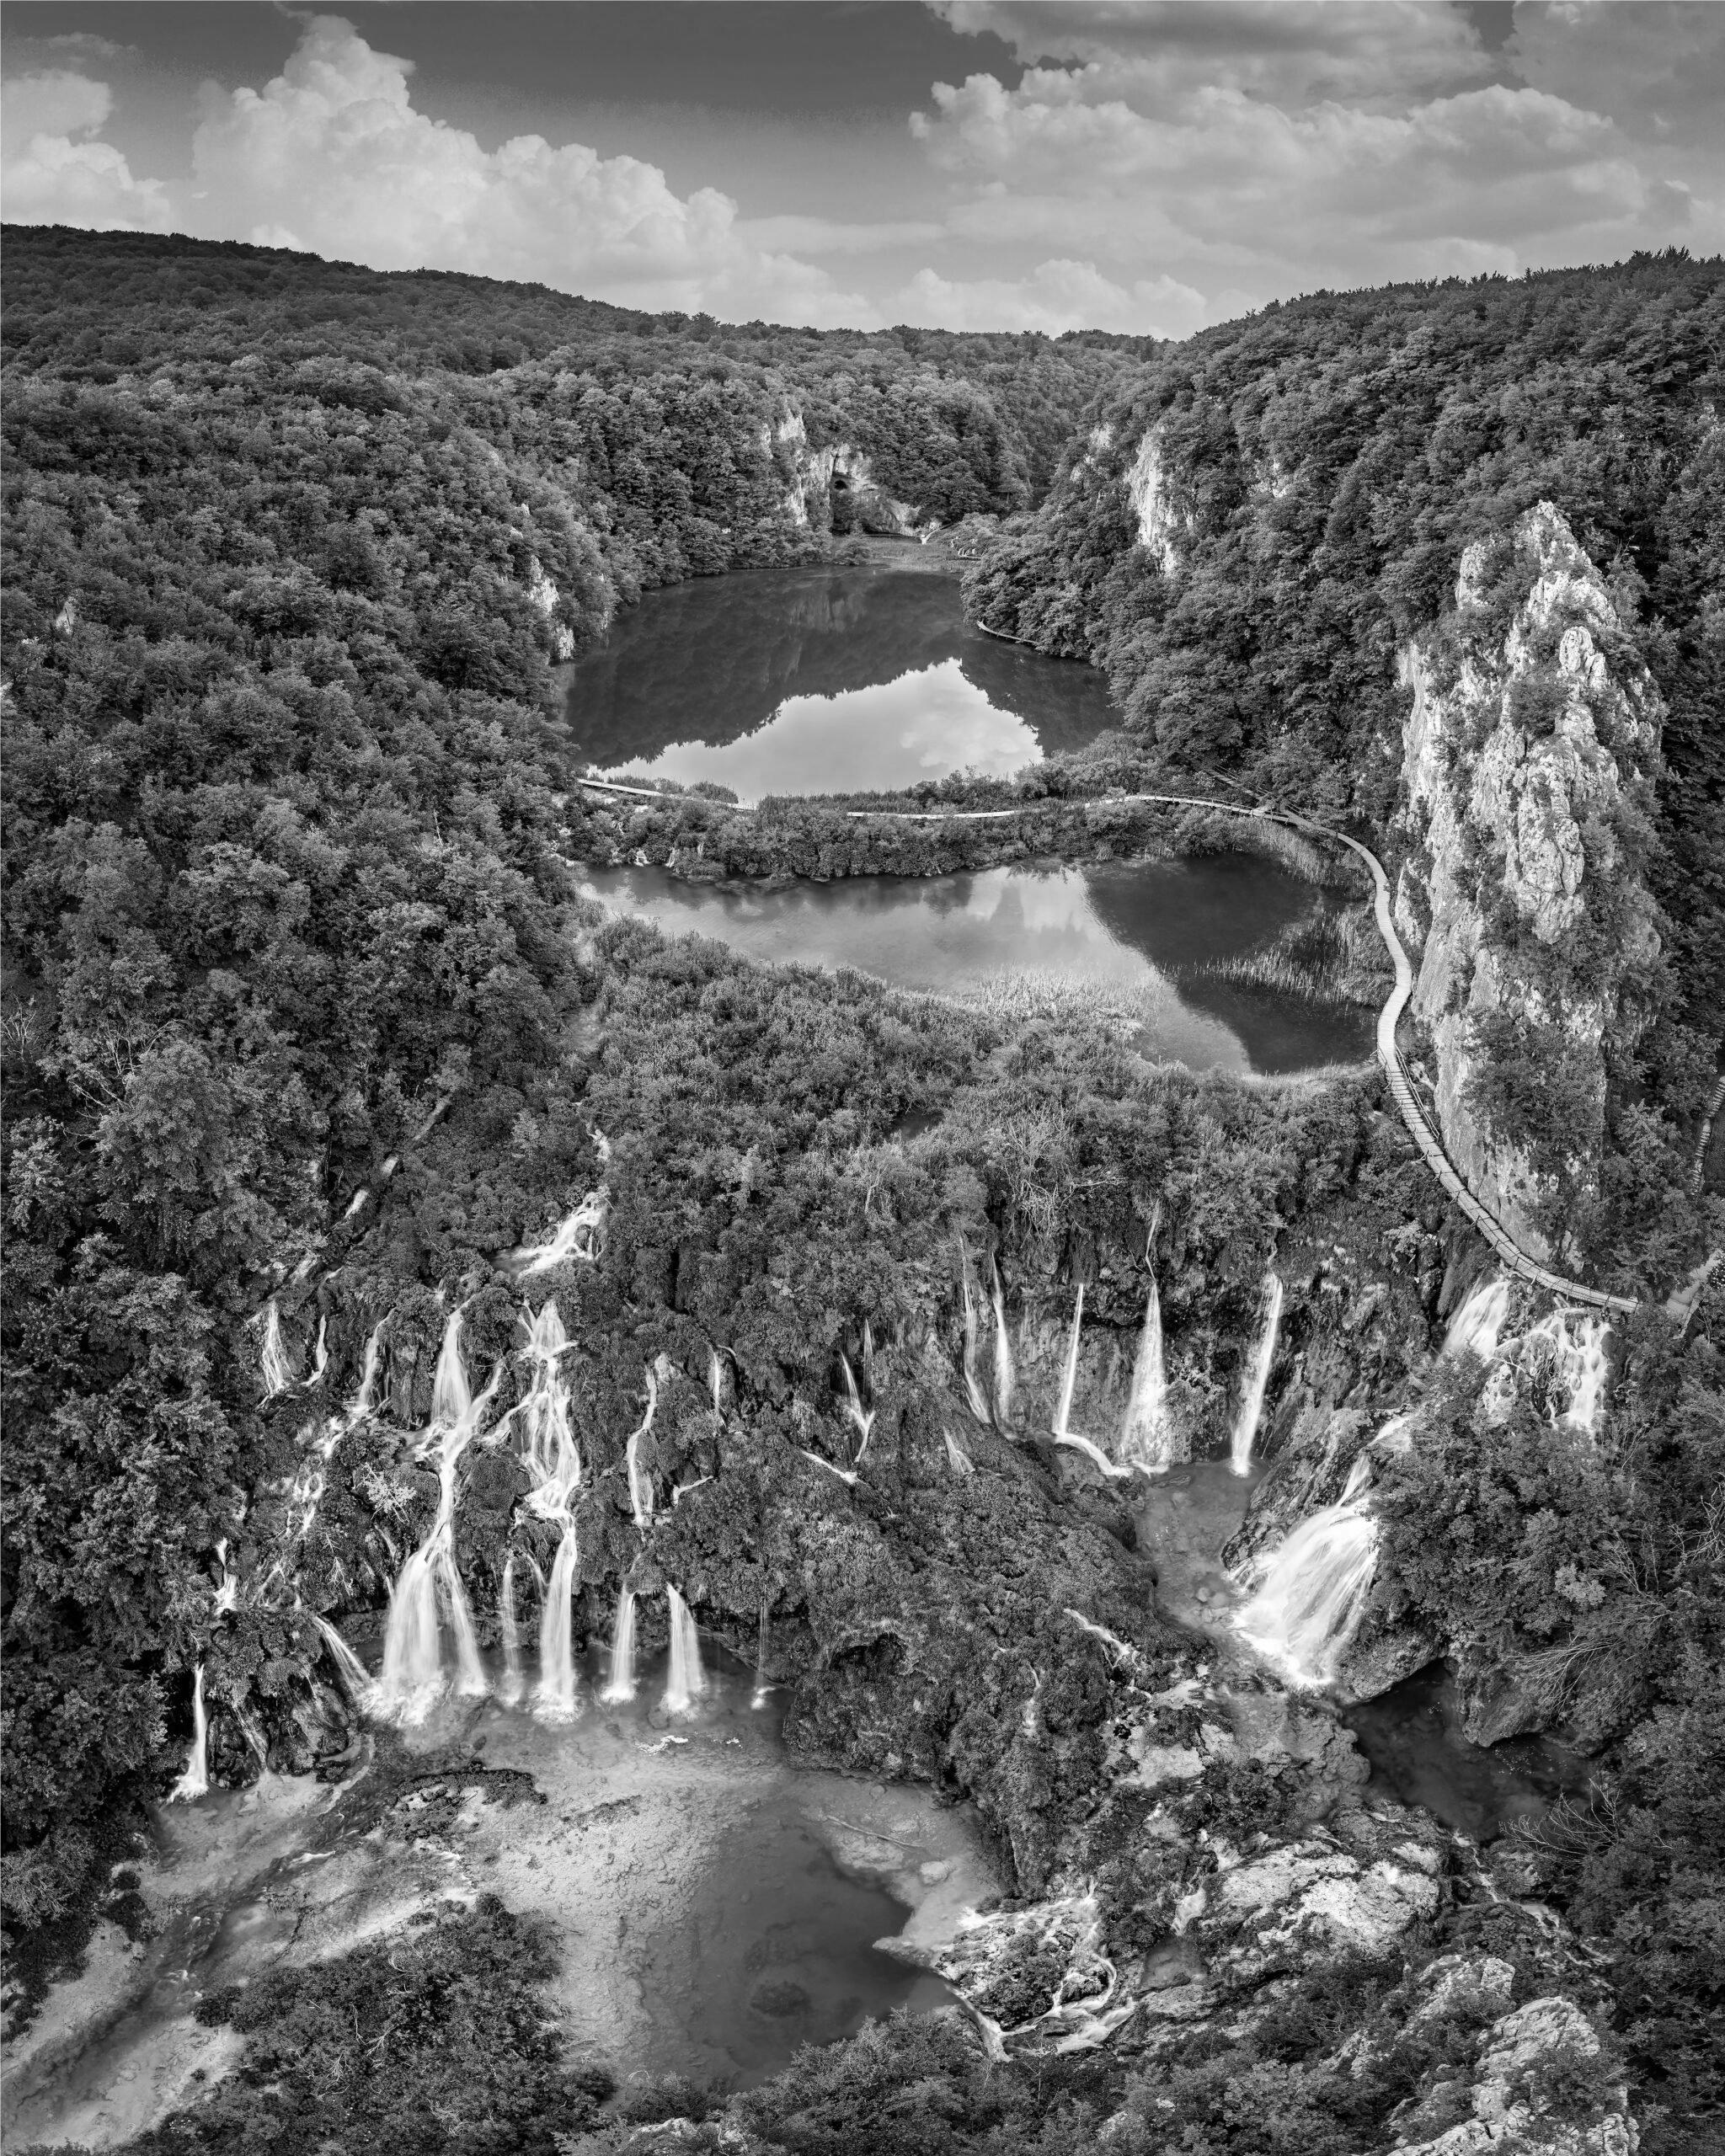
\includegraphics[width=0.7\linewidth]{slike/Grayscale.jpeg}
    \caption{Prikaz sive slike (vlastita izrada)}
\end{figure}

Na priloženoj sivoj slici se također može vidjeti da je različita od sivih slika kanala prikazanih na \hyperref[fig:channels]{slici 1}. To je zato što se kod pretvorbe slike u boji u sivu sliku uzimaju u obzir vrijednosti piksela za sva 3 kanala prema formuli:

{\large
\[
    I_{\text{siva}}(x, y) = 0.299 \cdot R(x, y) + 0.587 \cdot G(x, y) + 0.114 \cdot B(x, y)\text{\cite{Grayscale2}}
\]
}


\subsection{Binarne slike}

Osim slika u boji i sivih slika također postoje i binarne slike. Binarne slike su poseban tip slika gdje piksel može imati samo dvije moguće vrijednosti od kud im dolazi i naziv, te vrijednosti su nula ili jedan. Binarne slike sadrže puno manje informacija od ostalih tipova slika, ali isto tako smanjuju kompleksnost same slike i omogućuju fokusiranje na važne značajke slike. Baš zbog toga se jako često koriste kod obrada slika koristeći računalni vid \cite{BinarySlika}.

\begin{figure}[H]
    \centering
    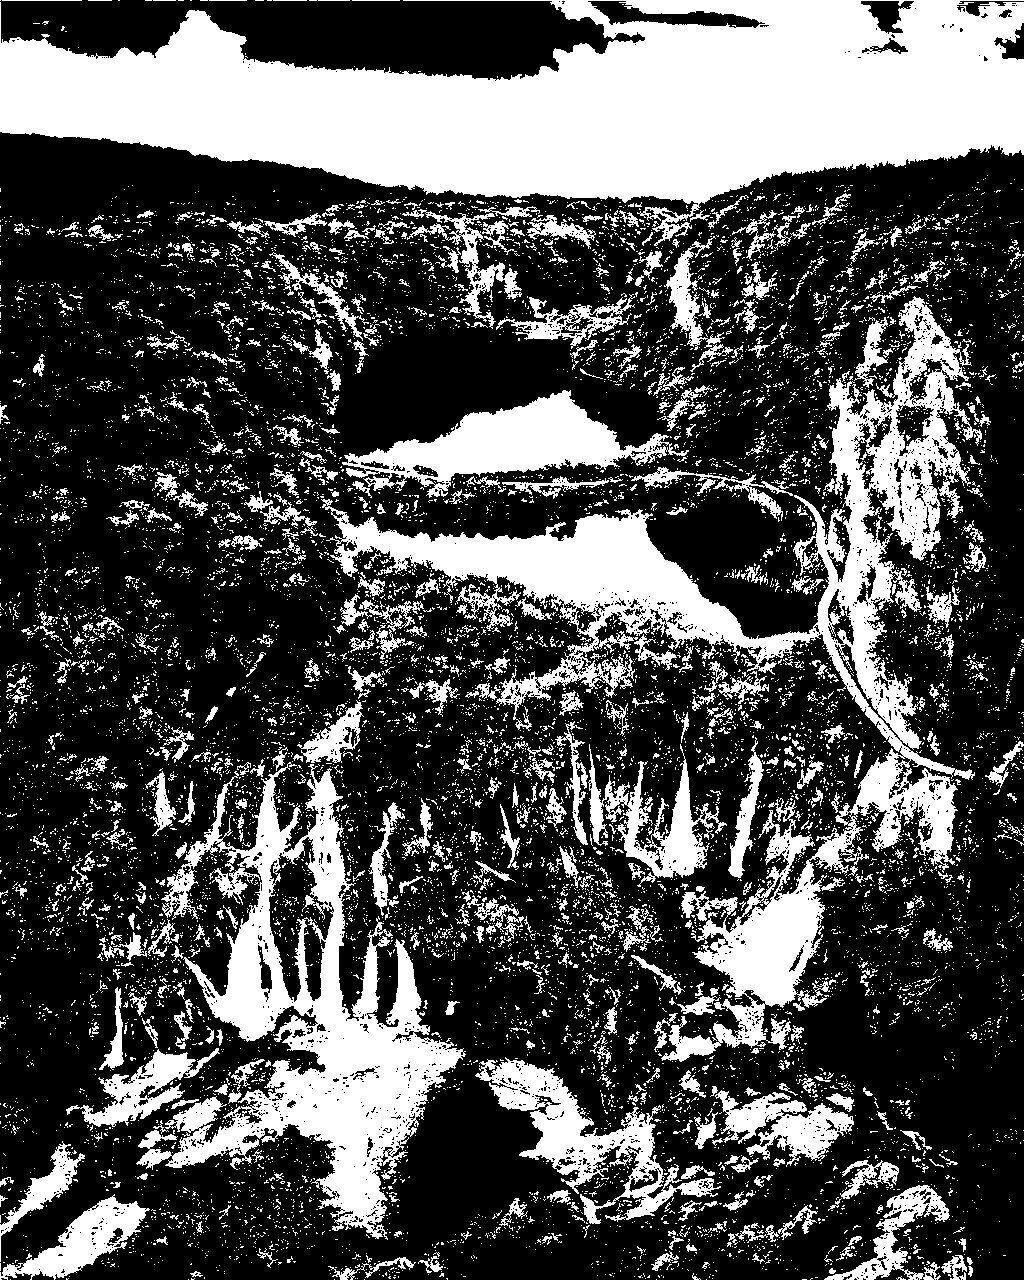
\includegraphics[width=0.75\linewidth]{slike/Binary.jpeg}
    \caption{Prikaz binarne slike (vlastita izrada)}
\end{figure}

Sam proces izrade binarne slike je dosta jednostavan. Za početak potrebno je imati sivu sliku. Zatim se definira granica (\textit{eng. threshold}) u obliku postotka ili vrijednosti piksela. Ta granica se zatim koristi za određivanje nove vrijednosti piksela, ako je vrijednost iznad granice onda se vrijednost postavlja na jedan, a inače na nulu. Priložena formula prikazuje osnovni tip kreiranja binarne slike (\textit{eng. tresholding}).

{\large
    \[
I_{\text{siva}}(x, y) = 0.299 \cdot R(x, y) + 0.587 \cdot G(x, y) + 0.114 \cdot B(x, y)
\]

\[
I_{\text{binarna}}(x, y) =
\begin{cases}
1, & \text{ako } I_{\text{siva}}(x, y) \geq T \\
0, & \text{ako } I_{\text{siva}}(x, y) < T
\end{cases}
\]}


\subsection{Važnost različitih tipova digitalnih slika}

Do sada smo prošli kroz 3 najvažnija tipa digitalnih slika za ovaj rad. Kroz ovu cjelinu prikazat će se važnost pojedinog tipa slike naspram ostalih.

Zapravo najveća razlika između ovih tipova je broj kanala boje. Slike u boji imaju 3 kanala za razliku od sivih i binarnih slika koje imaju po jedan kanal. To zapravo znači da slike u boji sadrže značajno više informacija. 

No ponekad nam te informacije nisu potrebne ovisno o problemu koji pokušavamo riješiti. Na primjer ako pokušavamo detektirati boju svjetla na semaforu onda su nam informacije o bojama izrazito važne. No ako pokušavamo pročitati tekst s prometnog znaka onda nam informacija o boji znaka i teksta ne doprinosi značajno rješavanju problema. Zapravo nam otežava rješavanje problema pošto moramo raditi s nepotrebnim informacijama.

\begin{figure}[H]
    \centering
    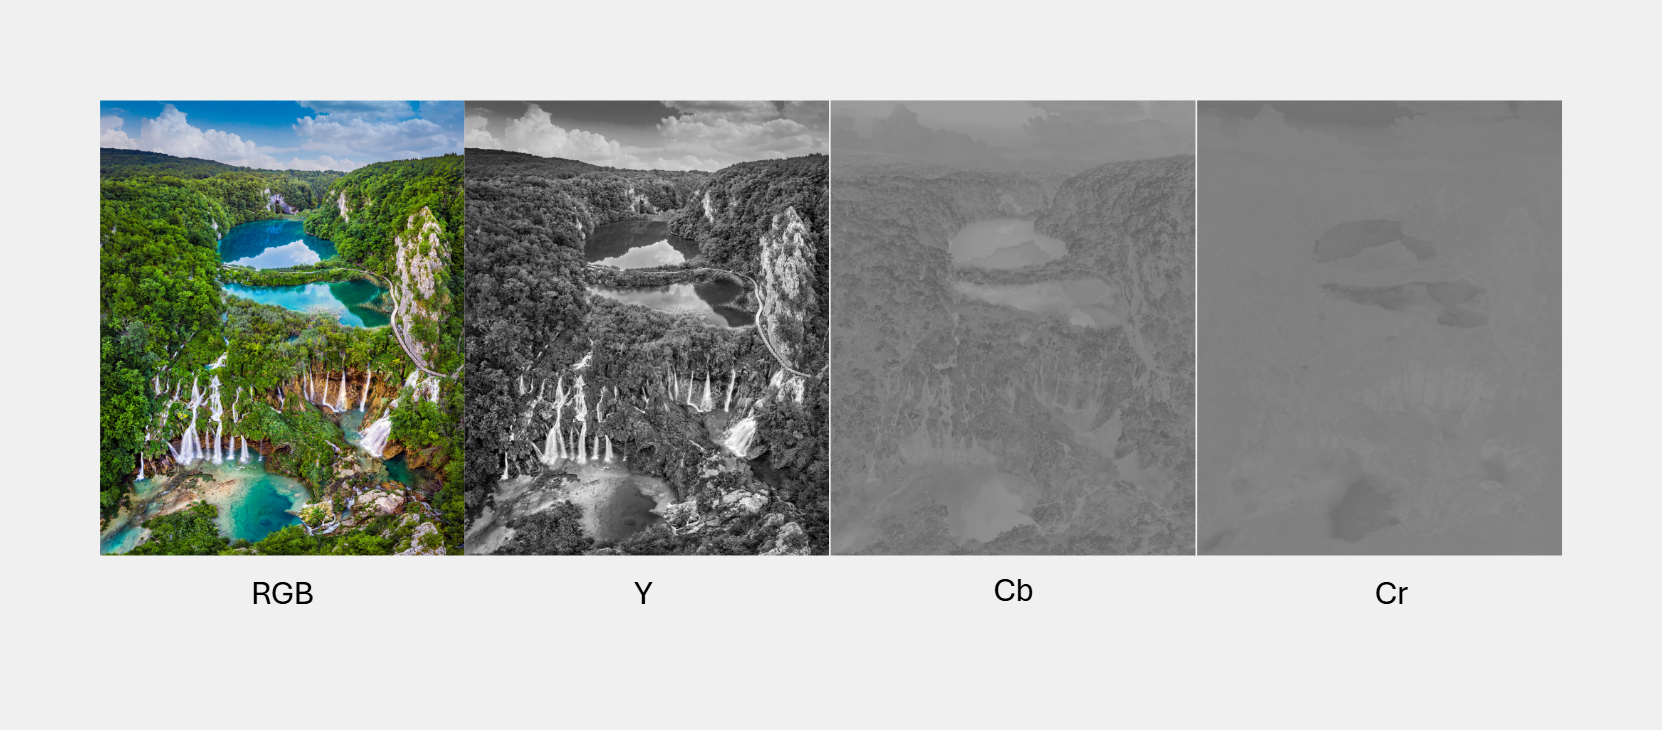
\includegraphics[width=1.0\linewidth]{slike/Luminace vs chrominance.png}
    \caption{Usporedba svjetlosne komponente i komponenta boja(vlastita izrada)}
\end{figure}

\begin{flushleft}
    Na priloženoj slici prikazana je ista slika na različite načine:
    \begin{itemize}[label=•]
        \item Slika u RGB formatu
        \item Slika u YCbCr formatu
        \begin{itemize}[label=•]
            \item Svjetlosne informacije u Y kanalu
            \item Informacije o bojama u Cb i Cr kanalima
        \end{itemize}
    \end{itemize}
    \end{flushleft}

Na ovom primjeru je prikazana činjenica da svjetlosni kanali sadrže puno više informacija o strukturnim elementima na slici. Baš zbog toga se u raznim algoritmima za detektiranje značajki, filtriranje, segmentiranje i sl. koriste baš sive slike \cite{LumVsChrom}. 

Sive slike se koriste kada boja nije važan faktor u obradi slike. U tom slučaju je boja jednako korisna kao buka na slici pa je zbog toga uklonimo. Time se veličina slike smanjuje i ujedno se ubrzava daljnji proces obrade slike \cite{LumVsChrom}.

Ako je potreban još agresivniji pristup otklanjanju nepotrebnih podataka, binarne slike mogu biti korisne. One dodatno odstranjuju nepotrebne podatke tako da povećavaju razliku u kontrastu i time odvajaju razne strukturne elemente slike \cite{LumVsChrom}.

Važno je napomenuti da svaki tip slika ima svoju upotrebu ovisno o problemu koji se rješava. U ovom radu će veliku važnost imati sive i binarne slike pošto se radi o procesu detektiranja strukture fotografije i izvlačenja relevantnih informacija iz nje.

\section{Digitalna obrada slike}

Digitalna obrada slike (\textit{eng. digital image processing}) podrazumijeva obradu digitalne fotografije koristeći računalne algoritme s ciljem unaprjeđivanja slike, izvlačenja korisnih informacija, analize, izrade izvještaja i slično. Predstavlja ključni korak u raznim primjenama računalnog vida temeljenog na dubokom učenju, poput prepoznavanja lica, detekcije objekata i optičke detekcije \cite{ImageProcessing}. 

\begin{flushleft}
Sam proces digitalne obrade slike može se podijeliti u sljedeće faze \cite{ImageProcessing}:
\begin{itemize}
\item Pribavljanje slike (\textit{eng. image acquisition})
\item Poboljšanje slike (\textit{eng. image enhancement})
\item Kompresija slike (\textit{eng. image compression})
\item Morfološka obrada (\textit{eng. morphological processing})
\item Segmentacija slike(\textit{eng. image segmentation})
\item Reprezentacija i opis (\textit{eng. representation and description})
\item Detekcija i prepoznavanje objekata (\textit{eng. object detection and recognition})
\end{itemize}
\end{flushleft}

Naravno nisu sve faze uvijek potrebne, već se radi o generalnim smjernicama koje se prema specifičnostima problema mogu modificirati, smanjiti ili proširiti. U nekim slučajevima čak se redoslijed faza može promijeniti ili se faze mogu provoditi više puta.    

Te faze se dodatno mogu podijeliti na \textbf{pretprocesiranje, procesiranje i postprocesiranje slike}. U fazu \textbf{pretprocesiranja} spadaju svi koraci koji pripremaju sliku za procesiranje, poput poboljšanja slike. Nakon pretprocesiranja slijedi \textbf{procesiranje} koje se odnosi na korištenje algoritama za detekciju i prepoznavanje objekata i transformacije. Posljednja faza uključuje korake poput pripreme rezultata za prezentaciju, vizualizaciju i daljnju analizu \cite{IamgeProcesingPhases}.

\pagebreak
\subsection{Pretprocesiranje slike}

Pretprocesiranje slike je ključan proces koji se provodi prije obrade slike. Kao ulaz prima izvornu, sirovu sliku, a kao izlaz vraća sliku u korisnijem formatu za daljnju obradu i analizu. Omogućuje da se sa slike odstrane ili istaknu područja relevantnih informacija te da se poboljša kvaliteta slike prije daljnje obrade \cite{Patel2023Oct}.

\subsubsection{Pribavljanje slike}

Pribavljanje slike je proces nastajanja digitalne slike tako da se informacije iz realnog svijeta zapišu u digitalnom obliku kojim računalo zatim može manipulirati. Slika se može pribaviti raznim uređajima poput fotoaparata, pametnog mobitela i drugih tehnologija poput skenera, rendgena. U ovom radu fokus će biti na fotografije pribavljene uređajima koji posjeduju digitalnu kameru \cite{BibEntry2025Apr}.


Da bi bilo kakvo procesiranje moglo krenuti, prvo je potrebno pribaviti sliku. Moglo bi se reći da je pribavljanje slike čak najvažniji korak u cijelom procesu obrade slike, njegov rezultat ima veliku ulogu za postizanje krajnjeg rezultata obrade i analize slike. Pribavljena slika mora biti kvalitetna da bi ostali koraci bili uspješni. Na kvalitetu slike ne utječe samo rezolucija, već osvjetljenje i kut pod kojim je slika uslikana također imaju značajnu ulogu \cite{BibEntry2025Apr}.

Razni algoritmi i koraci u pretprocesiranju mogu korigirati pribavljenu sliku, no to nikad nije zamjena za sliku dobre kvalitete. Dobra i loša slika mogu biti razlika između uspješnog i neuspješnog detektiranja elemenata na slici. Naravno u većini slučajeva sustavi za obradu slike ne mogu utjecati na kvalitetu slike koje će im korisnik poslati. Zbog toga je važno detaljno testirati sustav u različitim uvjetima i utvrditi što su njegove granice i je li potrebno podržati neki dodatni korisnički slučaj od onih postojećih.
\subsubsection{Poboljšanje slike}

Poboljšanje slike je ključan korak, cilj mu je modificirati sliku tako da ona postane korisnija za daljnju obradu. To se može postići na više načina poput otklanjanja buke, isticanja važnih značajki slike, poboljšanja oštrine i kontrasta slike.

Do sada smo spomenuli da se nepotrebne informacije na slici također mogu biti buka. Baš zbog toga pretvaranje u sivu i binarnu sliku spada pod poboljšanje slike. Oba dvije operacije uklanjaju nepotrebne informacije o bojama sa slike što omogućuje bržu i jednostavniju obradu i analizu slike. Naravno to ima smisla samo ako nam informacije o tim bojama nisu potrebne.

Osim nepotrebnih boja, bukom se može smatrati i nasumična razlika u vrijednosti između susjednih piksela. U digitalnoj fotografiji buka je praktički neizbježna i može se definirati kao nasumična varijacija signala u slici. Ta varijacija je reprezentirana različitim nijansama boja susjednih piksela. Buka se može smanjiti manipulacijom parametara digitalne kamera, ali ne može se kompletno ukloniti \cite{Adobe}.

Takve informacije se zbog malih razlika u boji piksela većinom mogu smatrati nevažnima, a loše utječu na daljnju obradu slike. Zbog toga postoje razne tehnike za filtriranje slike. Najpopularnije tehnike za filtriranje buke su \cite{Swain2023Jul}:

\begin{itemize}
    \item Gaussov filter (\textit{eng. gaussian filter})
    \item Srednji filter (\textit{eng. mean filter})
    \item Medijanski filter (\textit{eng. median filter})
    \item Bilateralni filter (\textit{eng. bilateral filter})
\end{itemize}


Svaki tip filtera ima svoju upotrebu i koristan je za određeni tip buke. Buka u digitalnim slikama je jako opširna tema koje se neće detaljnije objašnjavati u ovom radu.

\begin{figure}[H]
    \centering
    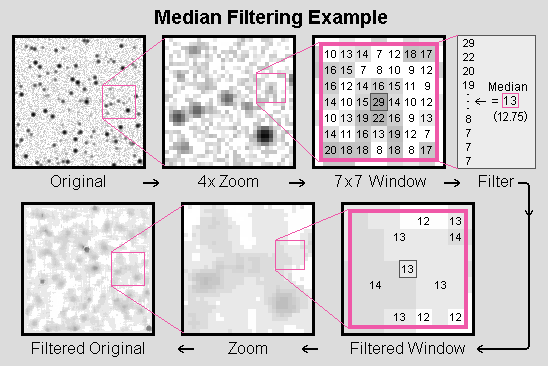
\includegraphics[width=0.85\linewidth]{slike/MedianFiltering.png}
    \caption{Primjer medijanskog filtera \cite{MeidanFilter}}
\end{figure}

Na priloženoj slici je prikazan proces korištenja medijanskog filtera koji naspram matrice susjednih vrijednosti određuje vrijednost piksela koristeći medijan svih vrijednosti.

Važno je napomenuti da su pojmovi poput oštrine i mutnoće  slike usko povezani s bukom. Jako često mutna slika sadrži manje buke, dok oštra slika može sadržavati više buke. Zbog toga je potrebno naći ravnotežu pri uklanjanju buke. Ako uklonimo previše buke, slika postaje mutna i gubi se previše informacija, obrnuto vrijedi ako uklonimo premalo buke.

Uklanjanje buke jedan je od najvažnijih koraka jer se nakon njega u daljnjim fazama ne analiziraju nepotrebne i neželjene informacije. Moglo bi se reći da je to de facto obavezan korak pretprocesiranja, budući da se izrazito često koristi.

\begin{figure}[H] 
    \centering 
    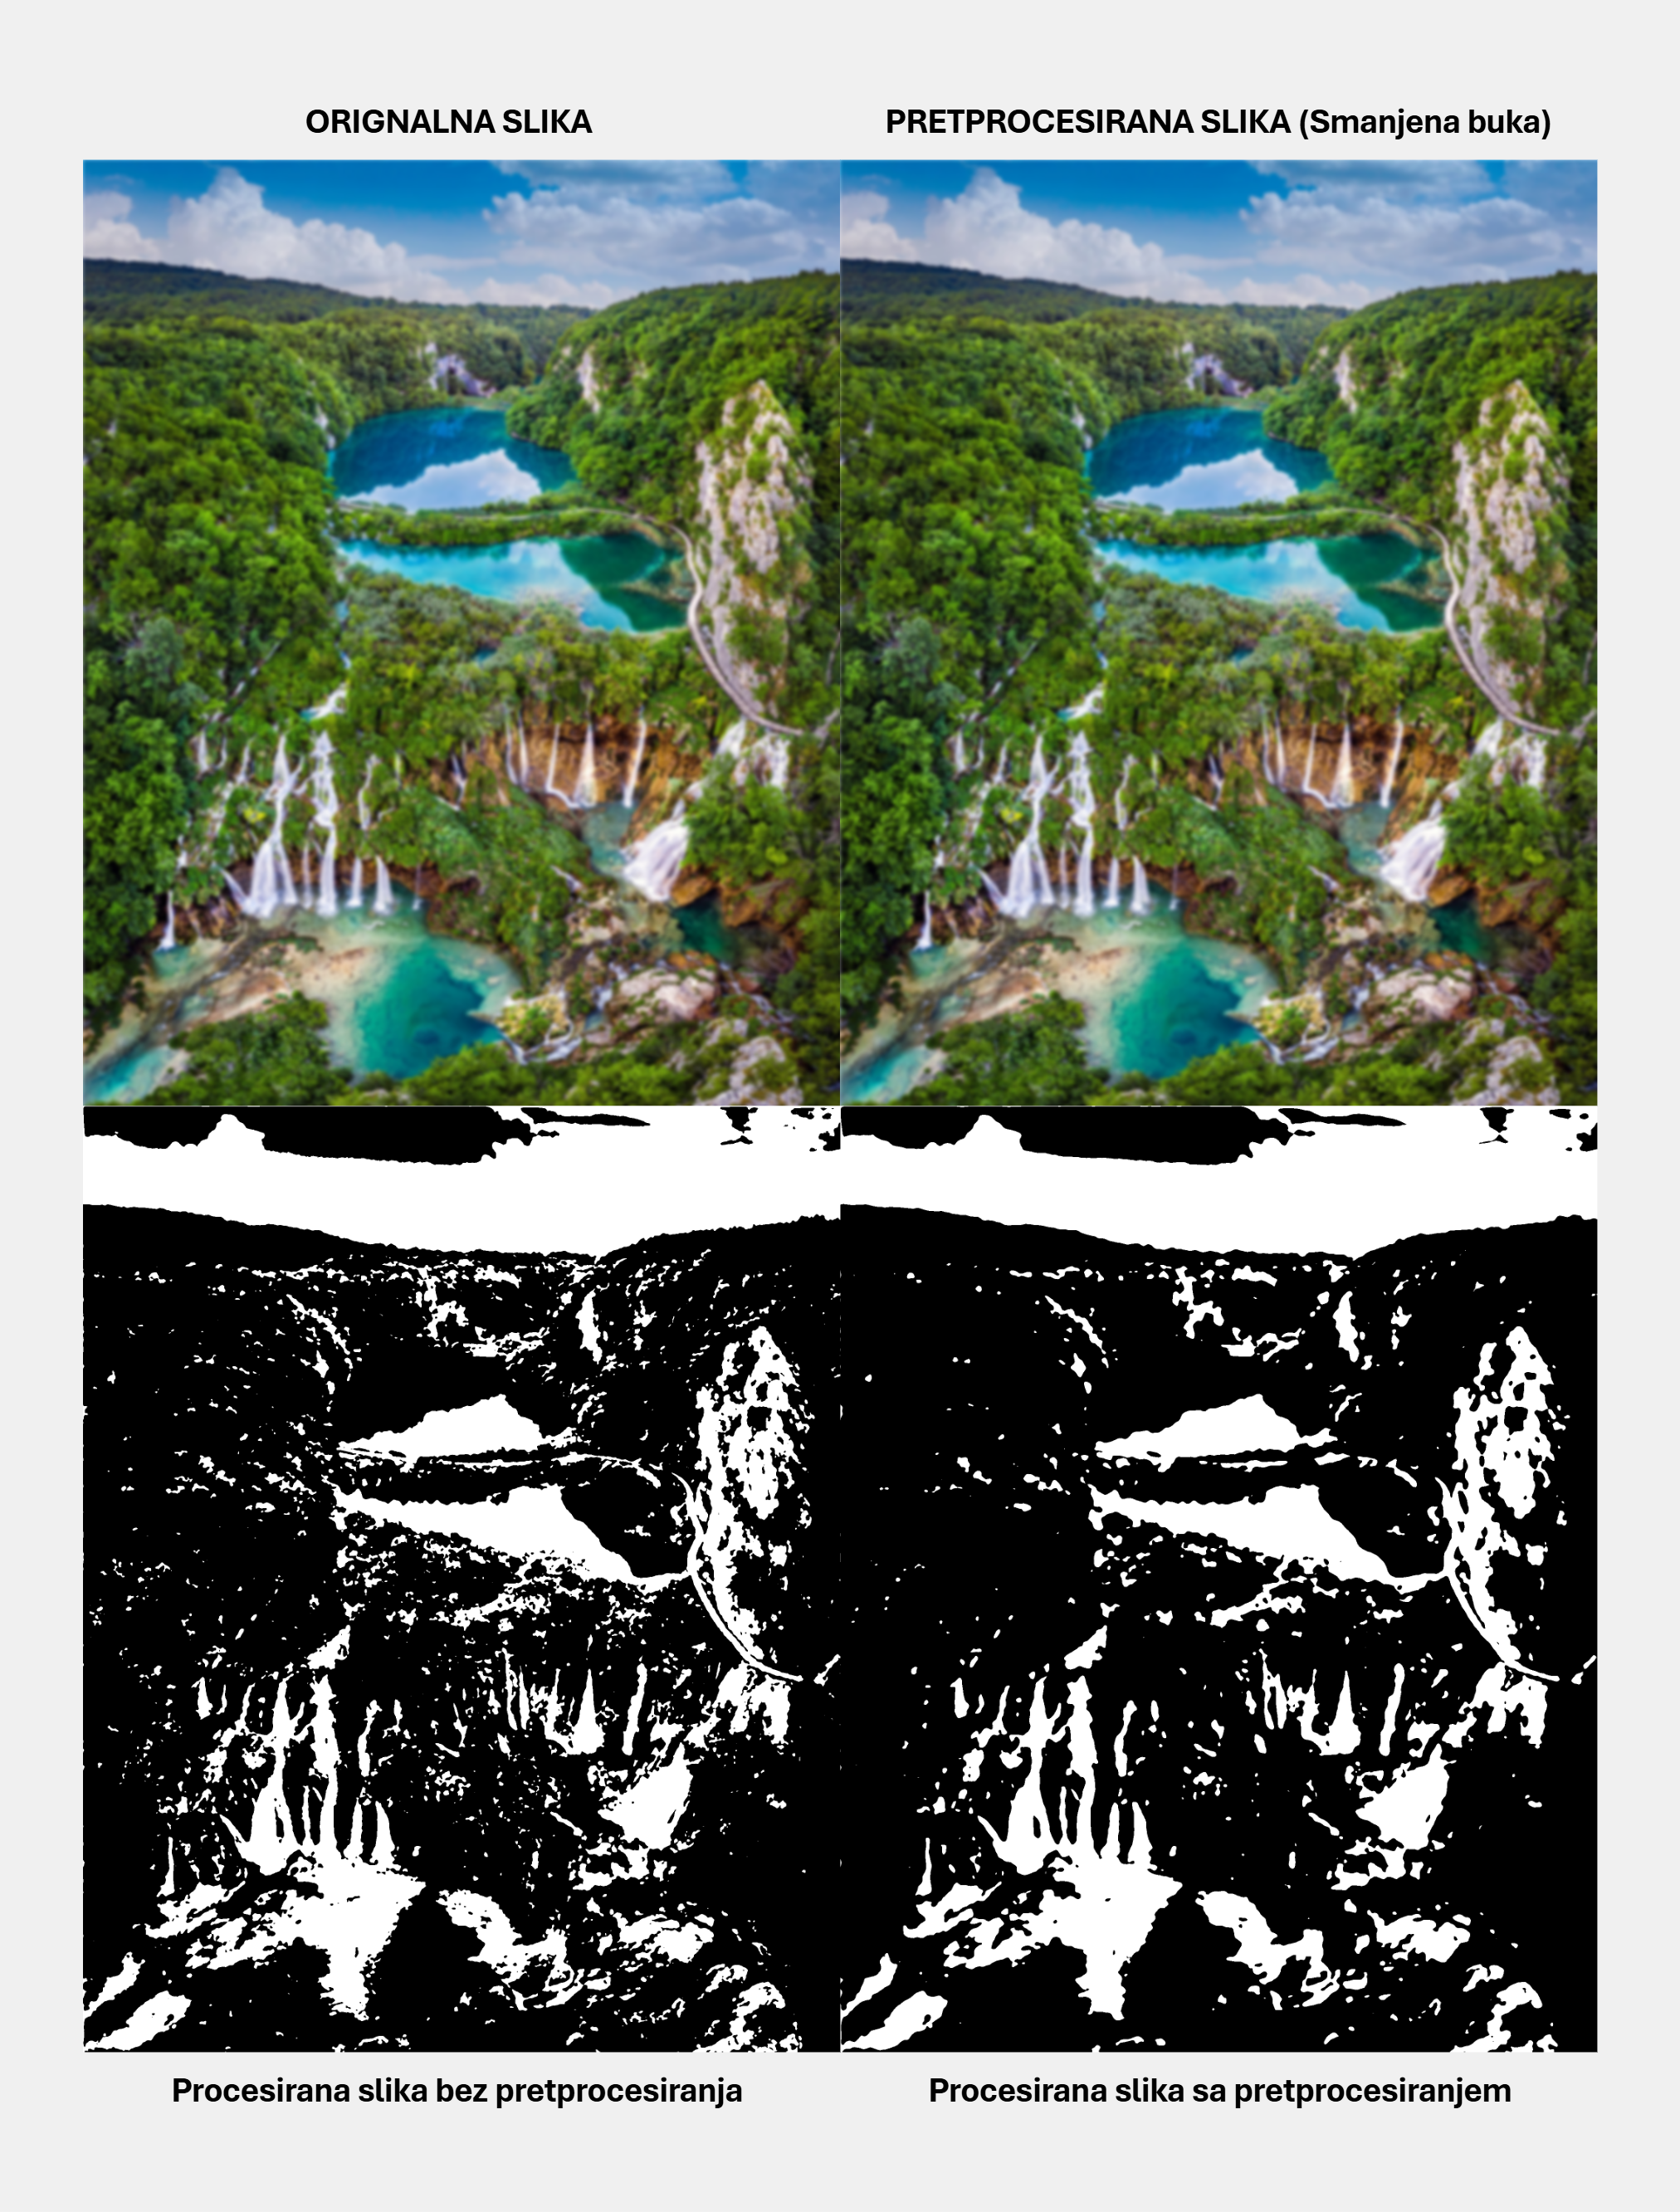
\includegraphics[width=0.85\linewidth]{slike/withAndWithoutPreProcessing.png} 
    \caption{Usporedba procesirane slike bez i s pretprocesiranjem (vlastita izrada)} 
\end{figure}

Na priloženoj slici moguće je vidjeti kako je znatno manje nevažnih informacija na desnoj binarnoj slici jer je pretprocesiranjem uklonjena buka, čime su dobiveni puno čišći podaci koji se mogu koristiti za daljnju obradu.

Postoji još razne metode poboljšavanja slike poput povećavanja kontrasta, ali neće biti potrebne u ovom radu.Također u nekim literaturama se spominju tehnike poput smanjenja buke  i raznih drugih transformacija u kontekstu restauracije slike. Ali u ovom radu će se o tome govoriti u kontekstu poboljšanja slike.

Druge važne metode poboljšavanja slike su razne geometrijske transformacije slike poput translacije, rotacije i skaliranja. Sve te osnovne geometrijske operacije koriste se kod ispravljanja perspektive. Baš zbog toga je ispravak perspektive puno zanimljivija operacija za ovaj rad \cite{GeometryTransforms}.

Ispravljanje perspektive omogućuje da slika prikazuje kao da je slikana u nekoj drugoj ravnini u prostoru. To omogućuje da se uklone neželjene značajke pribavljene slike poput kuta kamere naspram subjekta fotografije, u ovom slučaju papira s matricom odgovora. 

Korekcija perspektive mapira točku \( \mathbf{p} = [x, y, 1]^T \) u originalnoj slici (slikanoj iz nekog neželjenog kuta) \( \mathbf{p'} = [x', y', w']^T \) u sliku ispravljene perspektive s pomoću matrice \( H \) \cite{OpenCvPerpsective}.

\[
\mathbf{p'} = H \cdot \mathbf{p}
\]

Gdje \( H \) predstavlja \( 3 \times 3 \) homografsku matricu:

\[
H = 
\begin{bmatrix}
h_{11} & h_{12} & h_{13} \\
h_{21} & h_{22} & h_{23} \\
h_{31} & h_{32} & h_{33}
\end{bmatrix}
\]

Transformirane koordinate se računaju na sljedeći način:

\[
\begin{bmatrix}
x' \\
y' \\
w
\end{bmatrix}
=
\begin{bmatrix}
h_{11} & h_{12} & h_{13} \\
h_{21} & h_{22} & h_{23} \\
h_{31} & h_{32} & h_{33}
\end{bmatrix}
\cdot
\begin{bmatrix}
x \\
y \\
1
\end{bmatrix}
\]

Da bi te koordinate bile korisne potrebno ih je normalizirati s \( w \):

\[
x' = \frac{h_{11}x + h_{12}y + h_{13}}{h_{31}x + h_{32}y + h_{33}}, \quad
y' = \frac{h_{21}x + h_{22}y + h_{23}}{h_{31}x + h_{32}y + h_{33}}
\]

\begin{figure}[H]
    \centering
    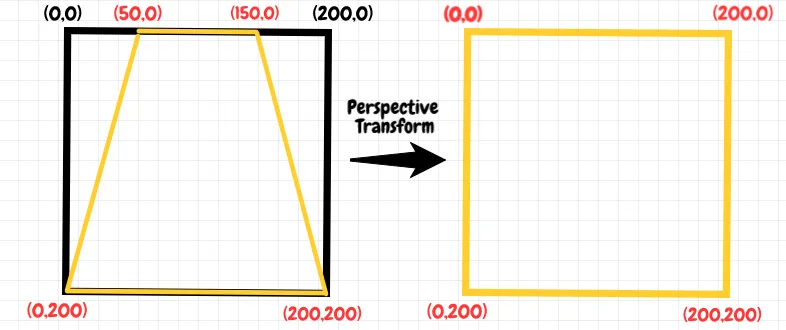
\includegraphics[width=0.85\linewidth]{slike/perspective.png}
    \caption{Prikaz procesa ispravka perspektive subjekta na slici \cite{OpenCvPerpsective}}
\end{figure}

Na priloženoj slici prikazano je kako se matrica transformacije koristi da bi se perspektiva ispravila. U praksi to funkcionira tako da se matrica transformacije računa naspram 4 izvorne i 4 odredišne točke. Te se zatim prema formuli množi sa svakom izvornom točkom da bi se izračunale odredišne točke.

\subsection{Procesiranje slike}

Nakon što je faza pretprocesiranja pretvorila sliku u korisniji format, kreće glavna faza obrade to jest procesiranje slike. Glavne tehnike kod procesiranja slike su segmentacija, detekcija objekata, morfološka obrada te reprezentacija i opis.

\subsubsection{Segmentacija slike}

Segmentacija slike je proces grupiranja piksela prema nekim obilježjima. Za razliku od običnih klasifikatora poput neuronskih mreža, segmentacija nudi informacije gdje se točno na slici nalazi objekt od interesa i koji su sve pikseli dio tog objekta. Isto kao u kod klasifikatora potrebno je definirati moguće klase kojima piksel može pripadati. Definiranje tih klasa može se učiniti na tri načina, prema kojima dijelimo tipove segmentacije na \cite{segmentacija}:

\begin{itemize}
    \item semantička segmentacija (\textit{eng. semantic segmentation })
    \item segmentacija instance (\textit{eng. instance segmentation})
    \item panoptička segmentacija (\textit{eng. panoptic segmentation})
\end{itemize}

\begin{figure}[H]
    \centering
    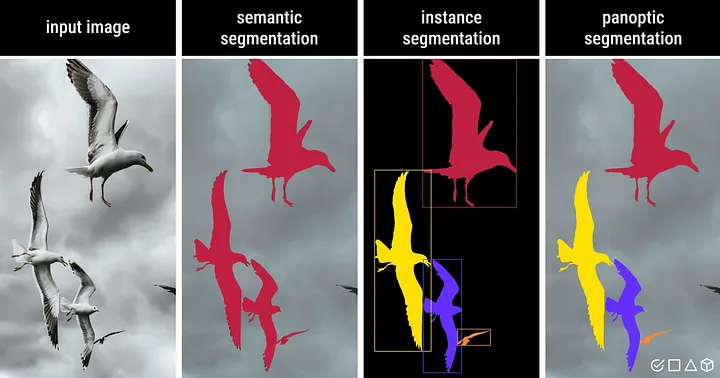
\includegraphics[width=0.85\linewidth]{slike/sesgmentacija.png}
    \caption{Usporedba tipova segmentacije \cite{segmentacija}}
\end{figure}

Na priloženoj slici definirane su dvije klase: nebo i ptice. Semantička segmentacija je sve piksele ptica klasificirala kao jednu klasu, što znači da ne znamo točno kojoj ptici pripada pojedini piksel. Da bi to riješili postoji segmentacija prema instanci što odvaja svaku pticu u zasebnu klasu što je bolje od semantičke, ali znači da više ne znamo koji sve pikseli pripadaju roditeljskoj klasi ptica. Da bi to riješili postoji panoptička segmentacija koja kombinira ta dva pristupa i pruža informacije o klasi piksela i kojoj instanci pripada. Tip segmentacije ovisi o specifičnostima problema koji se pokušava riješiti \cite{segmentacija}.


\subsubsection{Morfološka obrada}

Morfološka obrada je skup operacija koje procesiraju sliku. Omogućuje pronalazak elemenata na slici sličnih definiranom obliku. Usporedbu oblika vrši tako da traži grupu piksela koji odgovaraju tom obliku \cite{morph}.

Morfološka obrada se u nekim segmentima preklapa s segmentacijom slike, ali ne radi se o istim operacijama. Morfološke operacije se često koriste nakon segmentacije da uklone nedostatke iz detektiranih segmenata \cite{morph}.

Dvije najvažnije morfološke operacije su erozija i dilatacija.
Erozija funkcionira na način da uklanja piksele s ruba objekta. Vrlo je korisna u slučajevima kada je potrebno odvojiti dva objekta određenog oblika \cite{morph}. 

\begin{figure}[H]
    \centering
    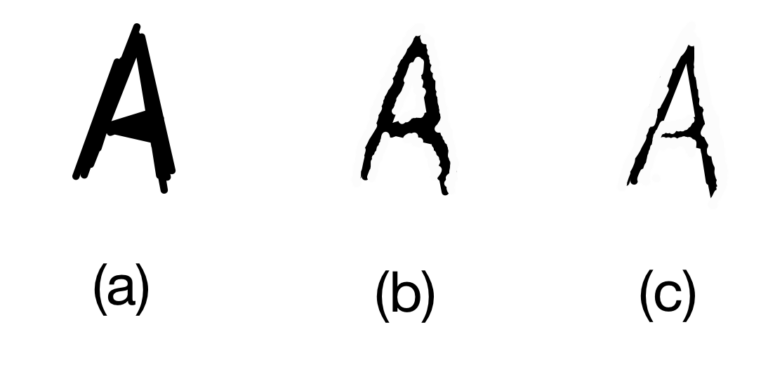
\includegraphics[width=0.75\linewidth]{slike/erosion.png}
    \caption{Prikaz erozije kao morfološke operacije \cite{morph}}
\end{figure}

Za razliku od erozije, dilatacija dodaje piksele oko ruba objekta. Time omogućuje da se popune praznine između objekata.

\begin{figure}[H]
    \centering
    
\includegraphics[width=0.75\linewidth]{slike/dilatacija.png}
    \caption{Prikaz dilatacije kao morfološke operacije \cite{morph}}
\end{figure}

Najčešće se te dvije operacije ne koriste zasebno već zajedno kao kompozitna morfološka operacija. Ako prvo provedemo eroziju, zatim dilataciju, radi se o otvaranju, dok obrnuti redoslijed operacija čini zatvaranje. \cite{morph}.

\begin{figure}[H]
    \centering
    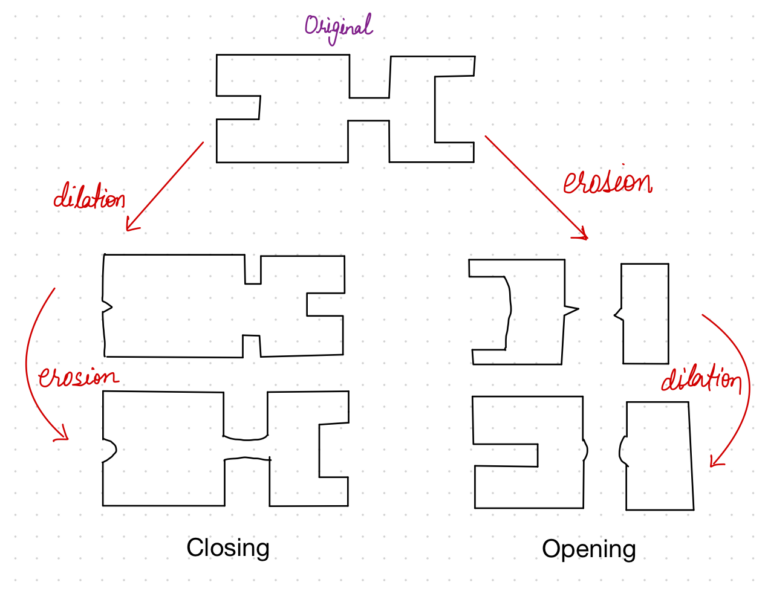
\includegraphics[width=0.6\linewidth]{slike/otvaranje_zatvaranje.png}
    \caption{Prikaz kompozitnih morfoloških operacija \cite{morph}}
\end{figure}

\subsubsection{Reprezentacija i opis}
Nakon što je obavljena segmentacija i po potrebi morfološka obrada većinom slijedi reprezentacija i opis segmentiranih dijelova. Cilj reprezentacije i opisa je reprezentirati piksele tako da budu korisniji za daljnju obradu \cite{RepAndDesc}. 

\begin{flushleft}
    Dva glavna tipa reprezentacije segmentiranih objekata, ovisno o tome je li fokus na \cite{RepAndDesc}:

\begin{itemize}
    \item vanjskim karakteristikama, (kontura ili rub objekta))
    \item unutarnjim karakteristikama (pikseli koji čine objekt)
\end{itemize}
\end{flushleft}

Reprezentacija prema vanjskim karakteristikama se često koristi kad nam je za obradu važan sam oblik, dok se unutarnje karakteristike koriste kada je potrebna informacija o boji i teksturi objekta. Iz dobivenih reprezentacija je moguće izvući razne opisne vrijednosti (\textit{eng. descriptors}) koje su korisne kod daljnje obrade. Važno je napomenuti da je generalno pravilo da bi opisne vrijednosti trebale biti imune na promjenu skaliranja, translacije i rotacije \cite{RepAndDesc}.

\begin{flushleft}
Neke od korisnik opisnih vrijednosti su \cite{RepAndDesc}:
\begin{itemize}
    \item Dužina konture objekta
    \item Promjer konture objekta
    \item Zaobljenost
    \item Okvirna kutija
    \item Površina objekta
    \item Sličnost željenom obliku
    \item Odstupanje od simetrije
    \item Koeficijent istezanja
\end{itemize}
\end{flushleft}

\subsubsection{Detekcija i prepoznavanje objekata}

Detekcija i prepoznavanje objekata je jedna od ključnih tehnika procesiranja slika na tradicionalan način, ali i s pomoću neuronskih mreža. Bazirano je na principu pronalaska objekta i crtanja okvirne kutije oko tog objekta \cite{segvsdetection, , segvsdetection_2}. 

To mu je ujedno i glavna razlika naspram segmentacije slike, segmentacija dodjeljuje klasu svakom pikselu koji odgovara onome što se traži, dok detekcija objekta to ne radi već samo locira objekt određene klase na slici \cite{segvsdetection, segvsdetection_2}.

Ponekad je samo informacija o lokaciji objekta dovoljna, u slučaju da nije segmentacija nudi puno više informacija o samom objektu.

Da bi detektiranje objekata bilo uspješno često se koriste konture. Konture su ništa drugo nego krivulje koje opisuju rubove objekata, zbog toga su jako korisne kod detektiranja oblika. Također se ponekad koriste i kod segmentiranja.

\begin{figure}[H]
    \centering
    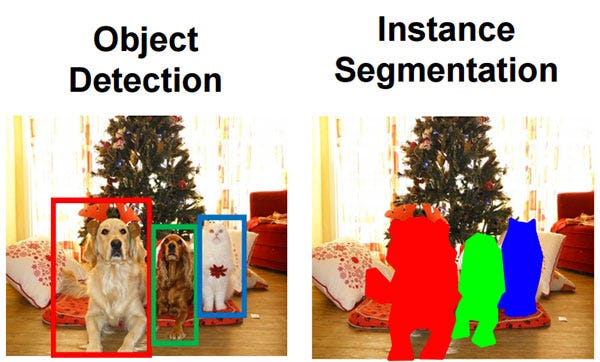
\includegraphics[width=0.6\linewidth]{slike/segVsDetec.png}
    \caption{Usporedba segmentacije i detekcije objekta \cite{segvsdetection_2}}
\end{figure}

Da bi se mogle pronaći konture prvo je potrebno sliku pretvoriti u binarnu sliku i zatim provesti operaciju detektiranja kontura. Konture se detektiraju tako da se traži razlika između kontrasta piksela na binarnoj slici i time se utvrđuje ujedno i granica između objekata. Zatim se primjenjuje jedna od metoda za detekciju objekta nad tim konturama. Te metode zapravo traže konture koje odgovaraju traženom obliku s definiranim tolerancijama za oblik, veličinu i slično \cite{konturesShapes}.

\begin{flushleft}
    Pošto će se u ovom radu koristiti EmguCv nama su najzanimljivije metode poput:
    \begin{itemize}
        \item \textbf{CvInvoke.ApproxPolyDP()} - Aproksimacija kontura u jednostavnije poligone (korisno za prepoznavanje oblika).
        \item \textbf{CvInvoke.MinAreaRect()} - Pronalaženje minimalnog pravokutnika koji okružuje konturu (korisno za detekciju objekata u obliku pravokutnika).
        \item \textbf{CvInvoke.FitEllipse()} - Fitting elipse na konturu (korisno za prepoznavanje eliptičnih objekata).
        \item \textbf{CvInvoke.HoughLinesP()} - Houghova transformacija za detekciju linija.
        \item \textbf{CvInvoke.HoughCircles()} - Houghova transformacija za detekciju krugova.
        \item \textbf{CvInvoke.BoundingRectangle()} - Pronalaženje okvira (bounding box) koji okružuje konture objekta.
        \item \textbf{CvInvoke.FindContoursHierarchical()} - Detekcija kontura s informacijama o hijerarhiji (za detekciju unutarnjih i vanjskih objekata).
    \end{itemize}
\end{flushleft}

\begin{figure}[H]
    \centering
    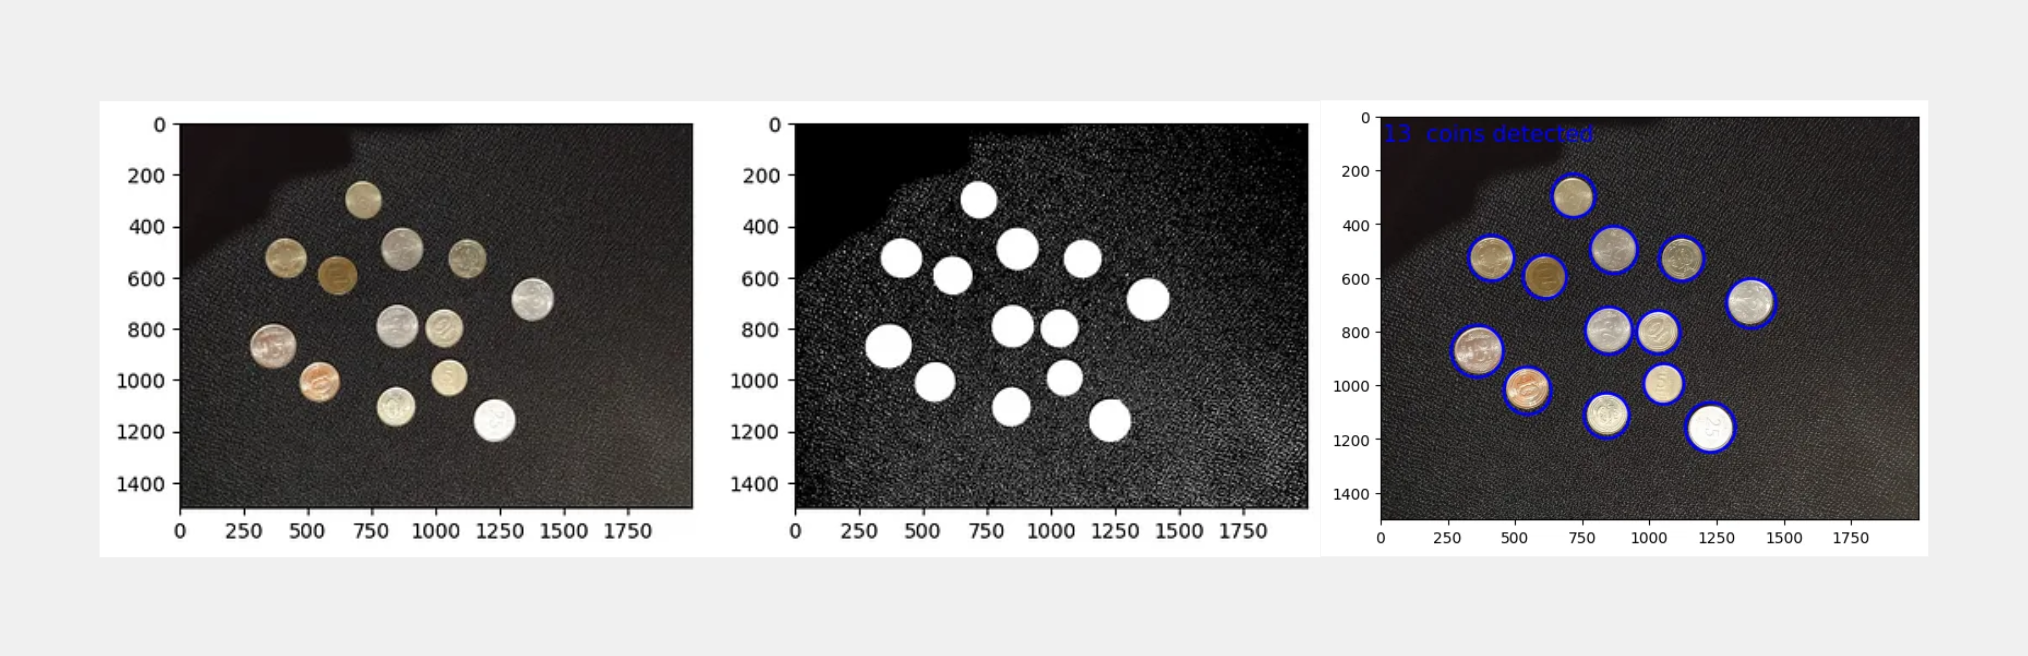
\includegraphics[width=1.0\linewidth]{slike/shapeDetection.png}
    \caption{\centering Prikaz rezultata detekcije krugova pomoću kontura i CvInvoke.MinEnclosingCircle metode \cite{segvsdetection_2}}
\end{figure}

Na priloženoj slici je jasno prikazano kako se izvorna slika pretvara u binarnu sliku i zatim se s pomoću kontura i metode za detektiranje oblika naspram kontura pronalazi lokacija kruga.

\subsection{Postprocesiranje slike}

Nakon što je glavna faza obrade slike završena kreću aktivnosti postprocesiranja. Prijašnja faza je izvukla korisne podatke iz slike i pripremila ih u korisnom formatu. Cilj postprocesiranje je obrada tih podataka tako da se dođe do konačnog rješenja. Osim obrade podataka, postprocesiranje je također povezano s aktivnostima poput vizualizacije rezultata, kompresije i slično.

\subsubsection{Obrada izvučenih podataka}

\begin{flushleft}
    Prije nego što se krene u konačnu obradu izvučenih podataka potrebno ih je pročistiti. Načini pročišćavanja podataka ovise o specifičnostima problema, ali neke od važnih metoda za ovaj rad su:
\begin{itemize}
    \item Filtriranje po veličini objekta
    \item Filtriranje po obliku objekta
    \item Filtriranje po boji objekta
    \item Filtriranje po hijerarhijskoj odnosu objekta s ostalim objektima
\end{itemize}
\end{flushleft}

Spomenute metode bazirane su na usporedbi opisnih vrijednosti iz faze reprezentacije i opisa. Nakon što su podaci pročišćeni kreće konačna faza obrade. Način konačne obrade ovisi o specifičnostima problema, ali često se koriste baze znanja.

Baze znanja omogućuju usporedbu traženih podataka s pročišćenim podacima koje omogućuje rješenje specifičnog problema. U ovom slučaju baza znanja bi bila lista odgovora za svako pitanje podijeljenih u dvije klase koje predstavljaju točne i netočne odgovore \cite{ImageProcessing}. 

\subsubsection{Vizualizacija rezultata}

Nakon što su podaci obrađeni i utvrđen je rezultat jako često ga je potrebno vizualizirati. Vizualizacija nudi uvid u njihovu važnost i omogućuje da se jednostavnije analiziraju i izvode zaključci iz rezultata. 
Tip vizualizacije ovisi o domeni problema koji se rješava. Može biti u raznim oblicima poput PDF izvješća, vizualizacije rezultata nad originalnom slikom i slično  \cite{Visulization}.

Kod vizualiziranja rezultata važno je uzeti u obzir tip podataka koji se vizualizira, publiku za koju je vizualizacija namijenjena \cite{Visulization}. 

\subsubsection{Kompresija slike}

U slučaju potrebe za smanjenjem veličine slike, često se koristi kompresija. Kompresija nastoji smanjiti veličinu slike na način da pritom zadrži kvalitetu na zadovoljavajućoj razini. Često se primjenjuje kada je potrebno smanjiti veličinu slike pri prijenosu preko mreže, spremanju u memoriju ili za ubrzanje obrade \cite{ImageProcessing}.

\begin{flushleft}
Kompresija slike dijeli se na dva glavna tipa \cite{Compression}:
\begin{itemize}
    \item Kompresija s gubitkom podataka (\textit{eng. lossy})
    \item Kompresija bez gubitka podataka (\textit{eng. lossless})
\end{itemize}
\end{flushleft}

Oba tipa smanjuju veličinu slike, ali se razlikuju u načinu na koji to postižu.  
Prvi pristup uklanja određene informacije iz slike kako bi smanjio njezinu veličinu (lossy), dok drugi pristup efikasnije zapisuje podatke bez gubitka informacija (lossless).  
Važno je napomenuti da je kod kompresije uvijek potrebno balansirati veličinu slike i kvalitetu. Što je slika više komprimirana, to je izraženija distorzija slike.  
Glavna razlika između ovih dvaju pristupa je u tome može li se originalna slika potpuno rekonstruirati iz komprimirane slike \cite{Compression}.

\pagebreak


\section{Analiza postojećih rješenja i pristupa problemu}

Prije praktičnog dijela rada važno je analizirati postojeća rješenja na tržištu. Ova analiza fokusirat će se samo na detekciju odgovora na pismenim ispitima koristeći matricu odgovora to jest detekciju OMR tehnikom (\textit{eng. optical mark recognition}). Pod OMR spadaju sve tehnike koje su do sada obrađene. Fokus analize je samo na rješenja visoke razine točnosti.

Osim korištenja računalnog vida uz OMR sve češći su pristupi koji koriste elemente dubokog učenja, samostalno ili u kombinaciji s tradicionalnim računalnim vidom \cite{OMRComparsion}.

Analizirana su rješenja OMRChecker i OpenOMR, radi se o rješenjima izrazito visoke točnosti koji tu točnost zadržavaju i kada je slika uslikana u izrazito izazovnim uvjetima. Također oba rješenja podržavaju određeni stupanj konfiguracije liste s odgovorima \cite{OMRComparsion}.

\begin{figure}[H]
    \centering
    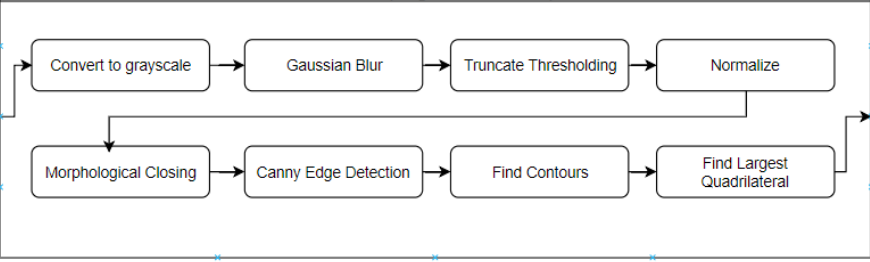
\includegraphics[width=1.0\linewidth]{slike/omr_flow.png}
    \caption{Prikaz dijela toka procesiranja slike kod OMRChecker-a \cite{OMRChecker}}
\end{figure}

S priložene slike vidljivo je da OMRChecker koristi veliku večinu metoda i tehnika koje su do sada obrađene u ovom radu, za OpenOMR je sitaucije također dosta slična.
Kroz praktični dio rada prikazat će se koji je cilj rješenja izrađenog u sklopu ovog rada i usporedit će se na kraju sa postojećim rješenjima.

\chapter{Praktični dio}

Kroz daljnji dio rada fokus će biti na izradi i prikazu komponente otvorenog koda za detekciju odgovora na pismenim testovima. Prikazat će se svi važni koraci i dizajnerske odluke koje utječu na konačni dizajn i funkcionalnost rješenja. Izrađena komponenta će također biti ugrađena u jednostavnu stolnu aplikaciju da bi se olakšalo razvoj i vizualizirao sam rad komponente. 

\section{Opis rješenja}

Kao što je već spomenuto cilj je izraditi komponentu otvorenog koda za detekciju odgovora na pismenim ispitima. Fokus će biti na detektiranju odgovora s matrice odgovora. Prednost toga pristupa je to što nije potrebno slikati više stranica da bi se ocijenio jedan ispit, već je dovoljno ocijeniti samo matricu odgovora, to jest obraditi samo jednu stranicu. 

Taj pristup detekciji odgovora je puno jednostavniji problem za riješavanje nego detekcija na standardnim ispitima. Jednostavniji je zbog toga što matrica može imati unaprijed definiranu i standardiziranu strukturu to jest predložak. Unatoč tome matrica limitira rješenje samo na pitanja s višestrukim ili jednostrukim odgovorima. No to nije problem za ovaj rad pošto drugi tipovi pitanja nisu u opsegu ovog rada.

Jedan od glavnih ciljeva ovog rješenja je da konzistentno pruža pouzdane rezultate, čak i ako uvjeti u kojima je slika uslika nisu idealni. Ta pouzdanost se treba postići za predloške koji mogu sadržavati varijabilan broj pitanja i odgovora. Da bi izrada predložaka bila što jednostavnija, rješenje bi također trebalo biti sposobno prema određenim parametrima generirati predložak matrice odgovora u obliku PDF-a. 

Također da bi se ubrzao rad s aplikacijom ideja je da korisnik ne unosi ručno podatke o točnim odgovorima za sva pitanja, već jednostavno slika ispravno riješen ispit te da komponenta sama izvuče te informacije iz fotografije. Da bi se dodatno ubrzao proces ocjenjivanja sustav treba biti dizajniran na način da detektirane odgovore usporedi s ispravnim odgovorima i ujedno prema korisnički definiranoj skali ocijeni ispit. Ocijenjeni ispit mora biti vizualiziran kako bi ocjenjivač mogao uvidjeti je li došlo do greške kod ocjenjivanja.

U svrhu bržeg razvoja, pronalaska grešaka i slično sustav bi trebao imati mogućnost vizualiziranja svakog koraka obrade od samog unosa slike pa sve do rješenja. Ta opcija bi se trebala moći uključiti ili isključiti po potrebi. 

Budući da se radi o komponenti otvorenog koda želja je da se ostavi mogućnost zamjene važnih biblioteka koje će sustav koristiti, poput one za računalni vid. Time će se omogućiti da netko po potrebi napiše svoju implementaciju i zamijeni zadanu EmguCv biblioteku.

\pagebreak

\section{Funkcionalni zahtjevi}


\begin{longtable}{|l|p{12cm}|}
    \hline
    \textbf{Identifikator} & FZ-01 \\ \hline
    \textbf{Zahtjev} & Sustav mora detektirati odgovore s matrice odgovora. \\ \hline
    \textbf{Opis} & Detekcija se temelji isključivo na obradi jedne stranice to jest matrice odgovora. Odgovori se trebaju detektirati, klasificirati prema tome jesu li označeni i zatim ih pridužiti odgovarajućem pitanju.\\ \hline
    \textbf{Način provjere} & Prilikom unosa slike matrice odgovora, sustav treba pravilno označiti sve odgovore na slici i označitiji ih odgovarajučom bojom ovisno o klasi kojoj pripadaju. \\ \hline
    \textbf{Prioritet [1--5]} & 5 \\ \hline
    \multicolumn{2}{|c|}{} \\ \hline
    
    \textbf{Identifikator} & FZ-02 \\ \hline
    \textbf{Zahtjev} & Sustav mora omogućiti generiranje PDF predložaka za matricu odgovora. \\ \hline
    \textbf{Opis} & Korisnici trebaju moći jednostavno izraditi matricu s unaprijed definiranim brojem pitanja i odgovora. \\ \hline
    \textbf{Način provjere} & Iz sustava treba biti moguće izvesti generirani predložak u PDF formatu, parametri za unos su broj pirtanja i broj odgovora po pitanju. \\ \hline
    \textbf{Prioritet [1--5]} & 3 \\ \hline
    \multicolumn{2}{|c|}{} \\ \hline
    
    \textbf{Identifikator} & FZ-03 \\ \hline
    \textbf{Zahtjev} & Sustav mora omogućiti automatsko prepoznavanje točnih odgovora iz slike ispravno riješenog ispita. \\ \hline
    \textbf{Opis} & Korisnik ne mora ručno unositi odgovore; slika ispravnog rješenja bit će dovoljna za generiranje ključa. \\ \hline
    \textbf{Način provjere} & Učitavanjem slike ispravno riješenog ispita sustav mora automatski prepoznati sve točne odgovore. \\ \hline
    \textbf{Prioritet [1--5]} & 4 \\ \hline
    \multicolumn{2}{|c|}{} \\ \hline
    
    \textbf{Identifikator} & FZ-04 \\ \hline
    \textbf{Zahtjev} & Sustav mora usporediti odgovore s točnim rješenjem i izračunati ocjenu prema skali koju je korisnik definirao. \\ \hline
    \textbf{Opis} & Automatsko ocjenjivanje ubrzava proces ispravljanja i smanjuje mogućnost pogreške. \\ \hline
    \textbf{Način provjere} & Nakon što se ispiti obrade, mora biti prikazana ocjena za svaki ispit u skladu sa skalom. \\ \hline
    \textbf{Prioritet [1--5]} & 4 \\ \hline
    \multicolumn{2}{|c|}{} \\ \hline
    \pagebreak
    \hline

    \textbf{Identifikator} & FZ-05 \\ \hline
    \textbf{Zahtjev} & Sustav mora omogućiti vizualizaciju rezultata ocjenjivanja za svakog korisnika. \\ \hline
    \textbf{Opis} & Omogućava ljudsku kontrolu rezultata i ispravnost prepoznavanja i ocjenjivanja. \\ \hline
    \textbf{Način provjere} & Vizualna prezentacija ispita s označenim točnim i netočnim odgovorima mora biti dostupna. \\ \hline
    \textbf{Prioritet [1--5]} & 3 \\ \hline
    \multicolumn{2}{|c|}{} \\ \hline
    
    \textbf{Identifikator} & FZ-06 \\ \hline
    \textbf{Zahtjev} & Sustav mora omogućiti prikaz svih koraka obrade slike. \\ \hline
    \textbf{Opis} & Korisnicima i developerima ova funkcionalnost je korisna za praćenje grešaka i ponašanja sustava. Slike se trebaju prikazati tijekom obrade i spremiti na disk računala. \\ \hline
    \textbf{Način provjere} & Funkcionalnost prikazuje korake i sprema ih na disk ako je uključena, inače ne. \\ \hline
    \textbf{Prioritet [1--5]} & 5  \\ \hline
    \multicolumn{2}{|c|}{} \\ \hline
    \textbf{Identifikator} & FZ-07 \\ \hline
    \textbf{Zahtjev} & Sustav mora podržavati pitanja s jednostrukim i višestrukim odgovorima. \\ \hline
    \textbf{Opis} & Korisnici trebaju imati mogućnost definiranja pitanja koja imaju jedan točan odgovor (jednostruki izbor) ili više točnih odgovora (višestruki izbor). Sustav mora pravilno detektirati i ocijeniti oba tipa pitanja. \\ \hline
    \textbf{Način provjere} & Prilikom testiranja, sustav mora ispravno ocijeniti ispite koji sadrže oba tipa pitanja. \\ \hline
    \textbf{Prioritet [1--5]} & 4 \\ \hline
    \caption{Funkcionalni zahtjevi}
\end{longtable}

\section{Nefunkcionalni zahtjevi}

\begin{longtable}{|l|p{12cm}|}
    \hline
    \textbf{Identifikator} & NFZ-01 \\ \hline
    \textbf{Zahtjev} & Sustav mora pružati pouzdane rezultate čak i u slučaju loših uvjeta pri snimanju (npr. sjenke, loš kontrast, zakrenutost). \\ \hline
    \textbf{Opis} & U praksi slike ispita neće uvijek biti idealne kvalitete, sustav mora biti sposoban obraditi sliku i u takvim uvjetima. \\ \hline
    \textbf{Način provjere} & Sustav se testira na uzorku slika s različitim uvjetima osvjetljenja, orijentacije i kvalitete. \\ \hline
    \textbf{Prioritet [1--5]} & 3 \\ \hline
    \pagebreak
    
    \hline
    \textbf{Identifikator} & NFZ-02 \\ \hline
    \textbf{Zahtjev} & Sustav mora omogućiti jednostavnu zamjenu vanjskih biblioteka poput one za računalni vid. \\ \hline
    \textbf{Opis} & Komponenta pruža sučelje koje korisnici mogu naslijediti i napisati svoju implementaciju i time zamijeniti biblioteku za CV. \\ \hline
    \textbf{Prioritet [1--5]} & 2 \\ \hline
    \multicolumn{2}{|c|}{} \\ \hline


    \textbf{Identifikator} & NFZ-03  \\ \hline
    \textbf{Zahtjev} & Sustav mora moći detektirati odgovore na predlošku s varijabilnim brojem pitanja i odgovora \\ \hline
    \textbf{Opis} & Korisnici će moći generirati predložak s različitim brojem pitanja i odgovora, sustav ih treba sve ispravno detektirati. \\ \hline
    \textbf{Način provjere} & Testirati s raznim kombinacijama matrica odgovora sposobnost detekcije kada broj pitanja i odgovora nije fiksan, već varijabilan. \\ \hline
    \textbf{Prioritet [1--5]} & 2  \\ \hline
    \multicolumn{2}{|c|}{} \\ \hline

    \textbf{Identifikator} & NFZ-04 \\ \hline
    \textbf{Zahtjev} & Sustav mora pronaći odgovore na slici unutar 500 milisekundi. \\ \hline
    \textbf{Opis} & Nakon što korisnik učita sliku i pritisne gumb za detekciju odgovora, sustav ima najviše 500 milisekundi za obradu slike i pronalazak odgovora. Ovo vrijedi za slike koje ne prelaze 4K rezoluciju. Vrijeme učitavanja slike (I/O operacije) nije uključeno u to ograničenje. \\ \hline
    \textbf{Način provjere} & Izmjeriti prosječno vrijeme potrebno za detekciju odgovora sa slike. \\ \hline
    \textbf{Prioritet [1--5]} & 1 \\ \hline
    
    \caption{Nefunkcionalni zahtjevi}
\end{longtable}

\section{Slučajevi korištenja}

Kroz dijagram slučajeva korištenja moguće je vidjeti koji su korisnici sustava te koja je razina njihove interakcije s određenim funkcijama i dijelovima sustava.
Važno je napomenuti da se radi o prikazu visoke razine, čiji elementi ne moraju nužno odgovarati programskom kodu jedan-na-jedan.
Na konkretnom primjeru ovog sustava može se uočiti da su ocjenjivači jedini korisnici. Oni imaju mogućnost iniciranja više različitih akcija unutar sustava.

\begin{figure}[H]
    \centering
    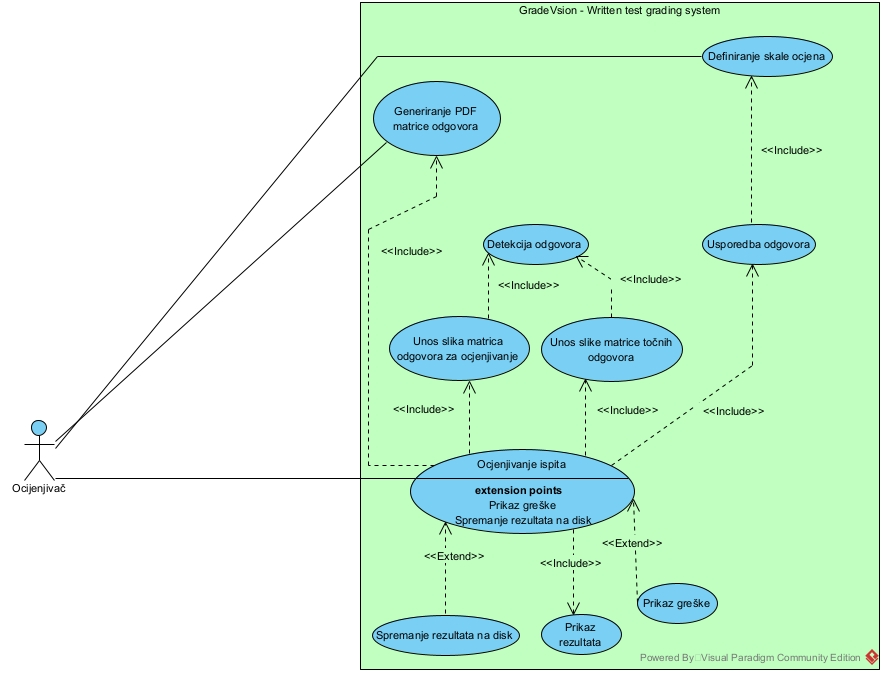
\includegraphics[width=1.0\linewidth]{slike/useCase.jpg}
    \caption{Prikaz Use-case diagrama (Vlastita izrada)}
\end{figure}

\subsection{Slučaj korištenja: Ocjenjivanje ispita}

\subsubsection{Korisnici}
Kao što je već spomenuto, ocjenjivači su jedini korisnici ovog sustava. Oni su u konačnici odgovorni za sam proces ocjenjivanja ispita, a GradeVision softversko rješenje im služi kao alat koji im u tom procesu značajno pomaže. Pomaže im tako što ubrzava sam proces ocjenjivanja, što im omogućuje da više vremena posvete ostalim obavezama, poput podizanja kvalitete nastave i sl.

\subsubsection{Glavni scenarij}
Glavni scenarij u ovom sustavu je ocjenjivanje ispita. Ocjenjivač pokreće tu aktivnost, koja zatim uključuje ostale dijelove sustava o kojima ovisi ispravan rad. To su druge aktivnosti poput generiranja PDF matrice odgovora, unosa slika i usporedbe odgovora.

\subsubsection{Uključeni slučaj uporabe: Generiranje PDF matrice odgovora}
Sustav ima mogućnost ocjenjivanja samo onih ispita koji imaju matrice odgovora u određenom formatu, stoga se prije ocjenjivanja ta matrica mora generirati. Taj format je donekle fleksibilan što se tiče broja pitanja i odgovora, ali osnovna struktura mora biti ista. Zbog toga ocjenjivač prije samog ocjenjivanja mora pokrenuti aktivnost "Generiranje PDF matrice odgovora" i definirati broj pitanja i odgovora kako bi kasnije mogao uspješno ocijeniti te matrice. Ako se ovaj korak preskoči i u sustav se učita matrica nekompatibilnog formata, sustav neće raditi.

\subsubsection{Uključeni slučaj uporabe: Unos slike matrice točnih odgovora}
Također, prije ocjenjivanja sustav mora znati koji su točni odgovori kako bi ih kasnije mogao usporediti. Stoga ocjenjivač mora učitati sliku matrice točnih odgovora čime se pokreće aktivnost "Unos slike matrice točnih odgovora".

\subsubsection{Uključeni slučaj uporabe: Unos slika matrica odgovora za ocjenjivanje}
Nakon što sustav ima učitanu sliku matrice točnih odgovora, potrebno je učitati slike matrica odgovora koje treba ocijeniti, jer bez tog koraka sustav ne zna što treba ocijeniti. Učitavanjem tih slika pokreće se aktivnost "Unos slika matrica odgovora za ocjenjivanje".

\subsubsection{Uključeni slučaj uporabe: Detekcija odgovora}
Obje aktivnosti učitavanja matrica odgovora ovise o aktivnosti "Detekcija odgovora", koja je ujedno jedna od najvažnijih aktivnosti koje sustav provodi, budući da se tu nalazi cijela logika za obradu slika i izdvajanje podataka o označenim odgovorima.

\subsubsection{Uključeni slučaj uporabe: Usporedba odgovora}
Nakon što su odgovori s učitanih matrica odgovora detektirani, pokreće se aktivnost "Usporedba odgovora", koja uspoređuje odgovore s matrica za ocjenjivanje s točnim odgovorima iz matrice točnih odgovora. Ta aktivnost također ovisi o aktivnosti "Definiranje skale ocjena", koja definira raspone za postizanje određene ocjene u postocima. U slučaju da skala nije definirana, koristi se unaprijed zadana skala.

\subsubsection{Ostali slučajevi uporabe}
Nakon što je ispit ocijenjen, pokreće se aktivnost "Prikaz rezultata", te po potrebi aktivnosti "Prikaz greške" i "Spremanje rezultata na disk". Zadnje dvije aktivnosti su opcionalne — spremanje na disk korisnik može uključiti ili isključiti, dok se greške prikazuju samo ako postoje razlike između detektiranih odgovora za ocjenjivanje i točnih odgovora. To mogu biti razlike poput različitog broja pitanja i odgovora i sl.

\subsubsection{Tijek aktivnosti}
\begin{flushleft}
Ovo je pravilan tijek aktivnosti slučaja korištenja "Ocjenjivanje ispita":
\begin{enumerate}
    \item \textbf{Generiranje PDF matrice odgovora} \\
    Ocjenjivač definira broj pitanja i odgovora te generira matricu u propisanom formatu.
    
    \item \textbf{Definiranje skale ocjena} \\
    Ocjenjivač može definirati vlastitu skalu ocjena. Ako se preskoči, koristi se zadana skala.
    
    \item \textbf{Unos slike matrice točnih odgovora} \\
    Učitava se slika ispravno riješenog ispita kako bi sustav prepoznao točne odgovore.
    
    \item \textbf{Unos slika matrica odgovora za ocjenjivanje} \\
    Učitavaju se slike ispita koje je potrebno ocijeniti.
    
    \item \textbf{Detekcija odgovora} \\
    Sustav obrađuje slike i izdvaja označene odgovore za svako pitanje.
    
    \item \textbf{Usporedba odgovora} \\
    Detektirani odgovori uspoređuju se s točnim odgovorima na temelju zadane skale ocjena.
    
    \item \textbf{Prikaz rezultata} \\
    Korisniku se prikazuju ocjene i vizualna oznaka točnih/netočnih odgovora.
    
    \item \textbf{Spremanje rezultata na disk (ako je uključena opcija)} \\
    Rezultati se mogu trajno pohraniti, ako je uključena ta opcija.
    
    \item \textbf{Prikaz greške (samo ako je potrebno)} \\
    Ako postoji nesukladnost između matrica (npr. broj pitanja), korisniku se prikazuje obavijest o grešci.
\end{enumerate}
\end{flushleft}


\section{Implementacija}
\section{Analiza rezultata}
\section{Limitacije rješenja}
\section{Manualno testiranje rješenja}
\chapter{Zaključak}

\printbibliography[title=Popis literature]
\addcontentsline{toc}{chapter}{Popis literature}

\listoffigures
\addcontentsline{toc}{chapter}{Popis slika}
 
\listoftables
\addcontentsline{toc}{chapter}{Popis popis tablica}

\appendix
\renewcommand{\thechapter}{\arabic{chapter}}


\end{document}